\chapter{State of the Art}
\label{state_of_art}
\linenumbers

\lettrine[lines=2]{I}{n coventional IT systems}, the objective of an attacker is to comprehend the behavior of a program using diverse techniques in order to launch attacks that alter its execution flow, functionalities, or bypass limitations imposed by software licensing. These attack techniques involve an initial examination of the program, consisting of \textit{static analysis} (i.e., analyzing the software without running it) and \textit{dynamic analysis} (i.e., analyzing the program while it is running).\newline 
The outcome of these two investigative techniques is the \textit{\textbf{reverse engineering}} of the software, which serves the purpose of identifying vulnerabilities or bugs and subsequently strategizing an attack.

\bigskip
In the context of OT systems, the notion of \textit{reverse engineering} is not limited to its conventional definition, but also includes the concept of \textbf{process comprehension}. This term, introduced by Green et al. \cite{green_et_al}, refers to gaining a comprehensive understanding of the underlying physical process.

\bigskip
There is limited literature available concerning the gathering and analysis of information related to the comprehension and operation of an Industrial Control System (ICS). In Section \ref{sec:3_related_work}, we will provide a brief overview of the existing literature on this topic, and in the subsequent sections, we will specifically focus on one of the presented papers.

\vfill

\section{Literature on Process Comprehension}
\label{sec:3_related_work}
\begin{description}
	\item[\textit{Keliris and Maniatikos}] The first approach presented in this section is by Keliris and Maniatakos \cite{keliris_maniatakos}: they present a methodology for automating the reverse engineering of ICS binaries based on a \textit{modular framework} (called ICSREF) that can reverse binaries compiled with CODESYS \cite{codesys}, one of the most popular and widely used PLC compilers, irrespective of the language used.
	
	\item[\textit{Yuan et al.}] Yuan et al. \cite{yuan_et_al} propose a \textit{data-driven} approach to discovering cyber-physical systems process behavior from data directly: to achieve this goal, they have implemented a framework whose purpose is to identify physical systems and transition logic inference, and to seek to understand the mechanisms underlying these processes, making furthermore predictions concerning their state trajectories based on the discovered models.
	
	\item[\textit{Feng et al.}] Feng et al. \cite{feng_swat} developed a framework that can generate system \textit{invariant rules} based on machine learning and data mining techniques from ICS operational data log. These invariants are then selected by systems engineers to derive IDS systems from them.\newline
	The experiment results on two different testbeds, the \textit{Water Distribution system} (WaDi) and the \textit{Secure Water Treatment system} (SWaT), both located at the iTrust - Center for Research in Cyber Security at the University of Singapore of Technology and Design \cite{itrust_site}, show that under the same false positive rate invariant-based IDSs have a higher efficiency in detecting anomalies than IDS systems based on a residual error-based model. 
	
	\item[\textit{Pal et al.}] Pal et al. \cite{pal_et_al} work is somewhat related to Feng et al.'s: this paper describes a data-driven approach to identifying invariants automatically using \textit{association rules mining} \cite{association_rules_mining} with the aim of generating invariants sometimes hidden from the design layout. The study has the same objective of Feng et al.'s and uses too the iTrust SwaT System as testbed.\newline
	Currently this technique is limited to only pair wise sensors and actuators: for more accurate invariants generation, the technique adopted must be capable of deriving valid constrains across multiple sensors and actuators.
	
	\item[\textit{Winnicki et al.}] Winnicki et al. \cite{winnicki_et_al} instead propose a different approach to process comprehension based on the \textit{attacker's perspective} and not limited to mere \textit{Denial of Service} (DoS): their approach is to discover the dynamic behavior of the system, in a semi-automated and process-aware way, through \textit{probing}, that is, slightly perturbing the cyber physical system and observing how it reacts to changes and how it returns to its original state. The difficulty and challenge for the attacker is to perturb the system in such a way as to achieve an observable change, but at the same time avoid this change being seen as a system anomaly by the IDSs.
	
	\item[\textit{Green et al.}] Green et al. \cite{green_et_al} also adopt an approach based on the attacker's perspective: this approach consists of two practical examples in a \textit{Man in the Middle} (MitM) scenario to obtain, correlate, and understand all the types of information an attacker might need to plan an attack to alter the process while avoiding detection.
	
	The paper shows \textit{step-by-step} how to perform a ICS \textbf{reconnaissance}, a phase specifically designed to gather extensive intelligence on multiple fronts, including human factors, network and protocol information, details about the manufacturing process, industrial applications, and potential vulnerabilities. The primary goal is to accumulate a wealth of information to enhance understanding and awareness in these areas \cite{ot_reconnaissance}).\newline 
	Reconnaissance phase is fundamental to process comprehension and thus to the execution of MitM attacks.
	
	\item[\textit{Ceccato et al.}] Ceccato et al. \cite{ceccato} propose a methodology based on a \textit{black box dynamic analysis} of an ICS using a reverse engineering tool to derive from the scans performed on the memory registers of the exposed PLCs and the Modbus protocol network scans an approximate model of the physical process. This model is obtained by inferring statistical properties, business process and system invariants from data logs.\newline
	The proposed methodology was tested on a non-trivial case study, using a virtualized testbed inspired by an industrial water treatment plant.
	
	In the next section we will examine this latest work in more detail, which will be the basis for my work and thus the subsequent chapters of this thesis.

\end{description}

\section{Ceccato et al.’s black-box dynamic analyisis for water-tank systems}
\label{sec:3_ceccato_metodology}
As previously mentioned, the paper introduces a methodology that relies on black box dynamic analysis of an Industrial Control System (ICS) and more particularly of its OT network. This methodology involves identifying potential Programmable Logic Controllers (PLCs) within the network and scanning the memory registers of these identified controllers. The purpose of this process is to obtain an approximate model of the controlled physical process.

\bigskip
The primary goal of this black box analysis is to establish a correlation between the different memory registers of the targeted PLCs and fundamental concepts of an OT network such as sensor values (i.e., measurements), actuator commands, setpoints (i.e., range of values of a physical variable), network communications, among others.\newline 
To accomplish this, the various types of memory registers are analyzed, and attempts are made to determine the nature of the data they might contain.\newline
The second goal is to establish a relationship between the dynamic evolution of these fundamental concepts.

\bigskip
To accomplish this, Ceccato et al. have developed a prototype tool \cite{plc_re} that facilitates the reverse engineering of the physical system. This tool goes through four distinct phases:

\begin{enumerate}
	\item \textbf{scanning of the system and data pre-processing}: this phase involves gathering data to generate data logs for the registers of PLCs and for Modbus network communications.
	
	\item \textbf{graphs and statistical analysis}: The collected data is utilized to provide insights into the memory registers associated with the Modbus protocol by leveraging graphs and statistical data. This analysis approach offers valuable information about the characteristics and patterns of the memory registers.
	
	\item \textbf{invariants inference and analysis}: generates system invariants, which are used to identify specific patterns and regularities within the system. Additionally, this phase provides users with the capability to view invariants related to a particular sensor or actuator.
	
	\item \textbf{business process mining and analysis}: Using event logs, this phase involves reconstructing the business process that depicts how a process is executed. This step enables a thorough understanding of the sequence of events that occur in the system and how they are interrelated, ultimately leading to a comprehensive overview of the business process.
\end{enumerate}

Figure \ref{fig:3_ceccato_overview} presents a schematic representation of the stages and the workflow associated with this work, specifying tools and technologies used. In the subsequent sections of this chapter, we will provide a detailed exploration of each of these phases, offering a comprehensive understanding of the entire process. 

\begin{figure}[ht]
	\centering
	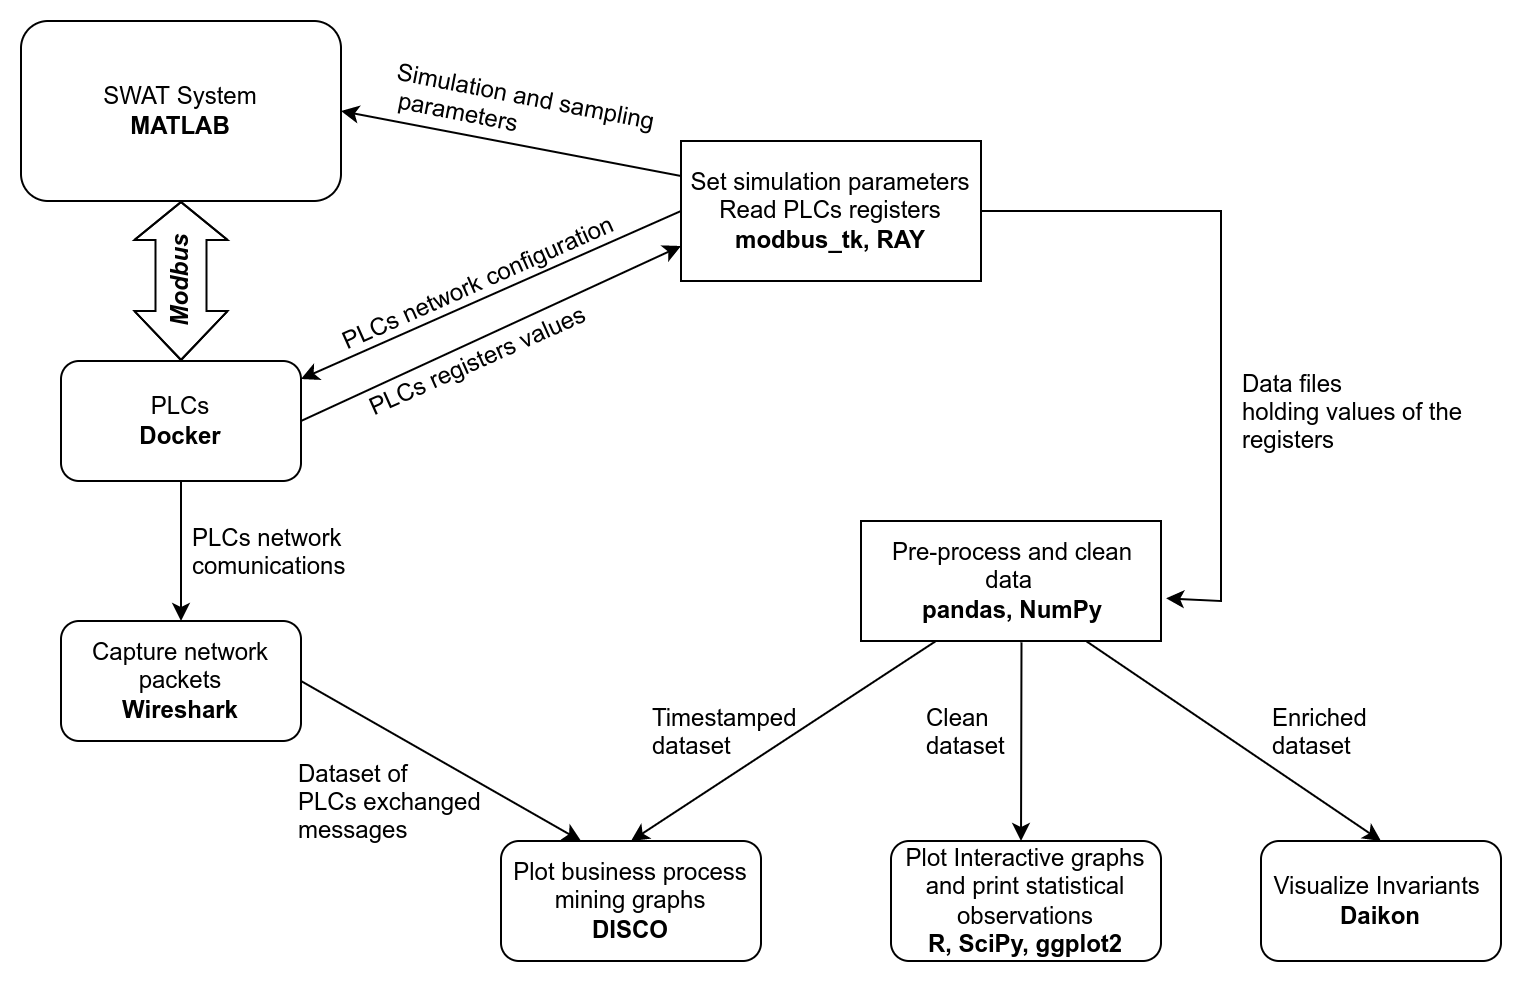
\includegraphics[scale=0.23]{chap3/ceccato_flowchart.png}
	\caption{Workflow of Ceccato et al.'s stages and operations with used tools}
	\label{fig:3_ceccato_overview}
\end{figure}

\subsection{Testbed}
\label{subsec:3_testbed}
Before delving into the description of the methodology's different phases, let's first examine the testbed utilized to evaluate this approach. The testbed employed for testing purposes is a (very) simplified rendition of the iTrust SWaT system \cite{swat_home}, as implemented by Lanotte et al. \cite{lanotte_et_al}. Figure \ref{fig:univr_testbed} provides a graphical representation of the testbed. This simplified version comprises three stages, each governed by a dedicated PLC.

\begin{figure}[ht]
	\centering
	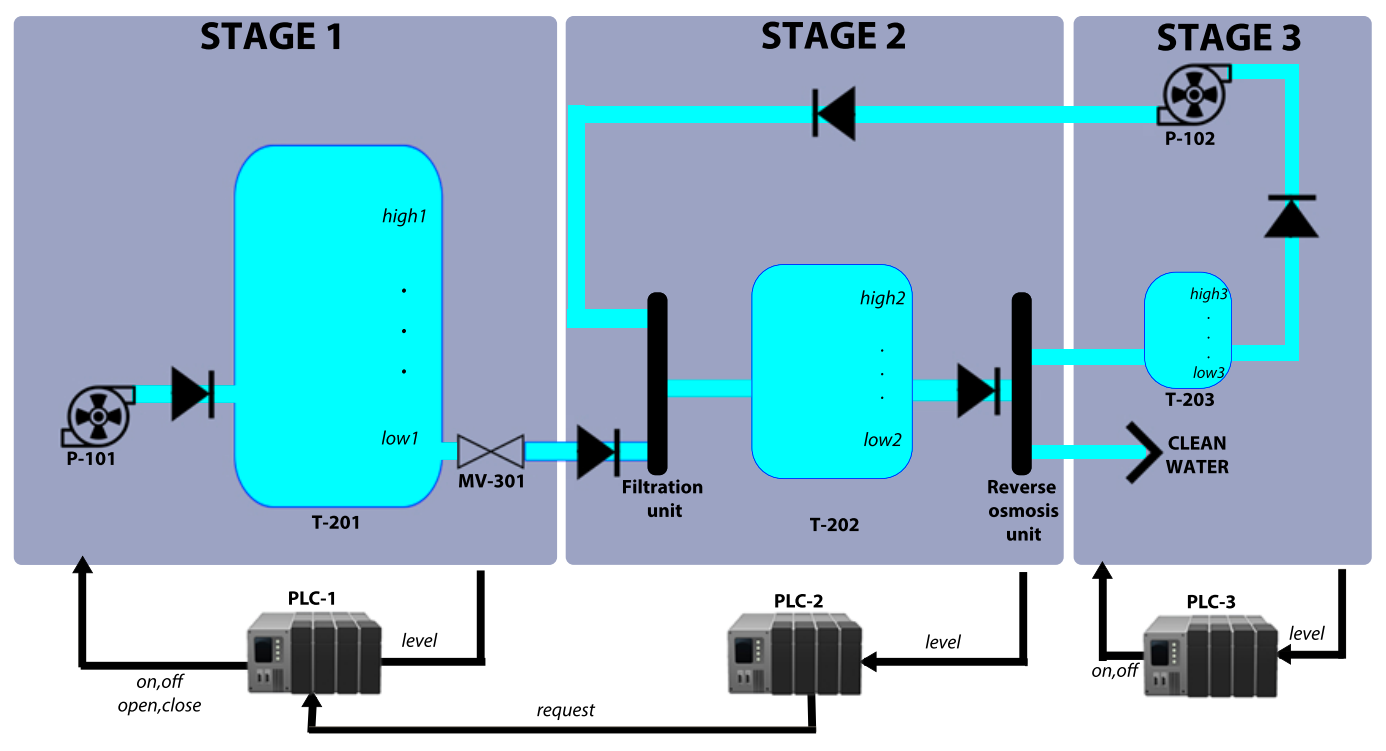
\includegraphics[scale=0.27]{chap3/univr_testbed.png}
	\caption{The simplified SWaT system used for running Ceccato et al. methodology}
	\label{fig:univr_testbed}
\end{figure}

\bigskip
\begin{description}
	\item[\textit{Stage 1}] During the initial stage, a \textbf{tank} referred to as T-201 with a capacity of 80 gallons is filled with raw water using the P-101 pump. Connected to the T-201 tank, the MV-301 motorized valve flushes out the accumulated water from the tank, directing it to the next stage. Initially, the water flows from the T-201 tank to the \textit{filtration unit} (which is not specifically identified by any sensor), and subsequently to a \textbf{second tank} denoted as T-202, with a capacity of 20 gallons.
	
	\item[\textit{Stage 2}] At the second stage, the water stored in tank T-202 flows into the \textit{reverse osmosis unit} (RO), which serves as both a valve and a continuous water extractor. The purpose of the RO unit is to reduce organic impurities present in the water. Subsequently, the water flows from the \textit{RO unit} to the third and final stage of the system.
	
	\item[\textit{Stage 3}] At the third stage, the water coming from the \textit{RO unit} undergoes division based on whether it meets the required standards. If the water is deemed clean and meets the standards, it is directed into the distribution system. However, if the water fails to meet the standards, it is redirected to a \textit{backwash tank} identified as T-203, which has a capacity of one gallon. The water stored in this tank is then pumped back to the stage 2 \textit{filtration unit} using pump P-102.
\end{description}

As previously mentioned, each stage of the system is handled via a dedicated PLC, namely PLC1, PLC2, and PLC3, which are responsible for controlling their respective stages. Let's briefly explore the behavior of each PLC:

\begin{description}
	\item[\textit{PLC1}] PLC1 monitors the level of tank T-201 and distinguishes three different cases based on the level readings:
	
	\begin{enumerate}
		\item when the level of tank T-201 reaches the defined \textit{low setpoint low1} (which is hardcoded in a specific memory register), PLC1 \textbf{opens pump P-101} and \textbf{closes valve MV-301}. This configuration allows the tank to be filled with water;
		
		\item if the level of T-201 reaches the \textit{high setpoint high1} (which is also hardcoded in a specific memory register), then the pump \textbf{P-101 is closed};
		
		\item in cases where the level of T-201 is between the \textit{low setpoint low1} and the \textit{high setpoint high1}, PLC1 waits for a request from PLC2 to open or close the valve MV-301. If a request to open the valve MV-301 is received, water will flow from T-201 to T-202. However, if no request is received, the valve remains closed. In both situations, the pump P-101 remains closed.
	\end{enumerate}

	\item[\textit{PLC2}] PLC2 monitors the level of tank T-202 and adjusts its behavior based on the water level. There are three cases to consider:
	
	\begin{enumerate}
		\item when the water level in tank T-202 reaches \textit{low setpoint low2} (also hardcoded in the memory registers), PLC2 sends a request to PLC1 through a Modbus channel to \textbf{open valve MV-301}. This request is made in order to allow the water to flow from tank T-201 to tank T-202. The transmission channel between the PLCs is established by copying a boolean value from a memory register of PLC2 to a corresponding register of PLC1.
		
		\item when the water level in tank T-202 reaches the \textit{high setpoint high2} value (also hardcoded in the memory registers), PLC2 sends a \textbf{close request to PLC1 for valve MV-301}. This request prompts PLC1 to close the valve, stopping the flow of water from tank T-201 to tank T-202.
		
		\item In cases where the water level in tank T-202 is between the low and high setpoints, the valve MV-301 remains in its current state (open or closed) while the tank is either filling or emptying.
	\end{enumerate}
	
	\item[\textit{PLC3}] PLC3 monitors the level of the T-203 backwash tank and adjusts its behavior accordingly. There are two cases to consider:
	
	\begin{enumerate}
		\item If the water level in the backwash tank reaches the \textit{low setpoint low3}, \textbf{PLC3 sets pump P103 to off}. This allows the backwash tank to be filled.
		
		\item If the water level in the backwash tank reaches the \textit{high setpoint high3}, \textbf{PLC3 opens pump P103}. This action triggers the pumping of the entire content of the backwash tank back to the filter unit of T-202.
	\end{enumerate}
\end{description} 

%%% SONO ARRIVATO QUI CON CHATGPT %%%

\subsection{Scanning of the System and Data Pre-processing}
\label{subsec:3_scan_preproc}
\paragraph{Scanning tool}
\label{par:3_scanning_tool}
The Ceccato et al. scanning tool extends and generalizes a project I did \cite{ns_proj} for the "\textit{Network Security}" and "\textit{Cyber Security for IoT}" courses taught by Professors Massimo Merro and Mariano Ceccato, respectively, in the 2020/21 academic year. The original project involved, in its first part, the recognition within a network of potential PLCs listening on the standard Modbus TCP port 502 using the Nmap module for Python, obtaining the corresponding IP addresses: then a (sequential) scan of a given range of the memory registers of the found PLCs was performed to collect the register data. The data thus collected were saved to a file in \textit{JavaScript Object Notation} (JSON) format for later use in the second part of my project.

\bigskip
The scanning tool by Ceccato et. al works in a similar way, but extends what originally did by trying to discover other ports on which the Modbus protocol might be listening (since in many realities Modbus runs on different ports than the standard one, according to the concept of \textit{security by obscurity}) and, most importantly, by \textbf{parallelizing and distributing the scan} of PLC memory registers through the Ray module \cite{ray}, specifying moreover the desired granularity of the capture. An example of raw data capture can be seen at Listing \ref{lst:raw_registers_capture}:

\begin{lstlisting}[language=Python, numbers=none, caption=Example of registers capture, label=lst:raw_registers_capture]	
	"127.0.0.1/8502/2022-05-03 12_10_00.591": {
		"DiscreteInputRegisters": {"%IX0.0": "0"},
		"InputRegisters": {"%IW0": "53"},
		"HoldingOutputRegisters": {"%QW0": "0"},
		"MemoryRegisters": {"%MW0": "40","%MW1": "80"},
		"Coils": {"%QX0.0": "0"}}
\end{lstlisting}
The captured data includes PLC's IP address, Modbus port and timestamp (first line), type and name of registers with their values read from the scan (subsequent lines).

\bigskip
The tool furthermore offers the possibility, in parallel to the memory registers scan, of \textbf{sniffing network traffic} related to the Modbus protocol using the \textit{Man in the Middle} (MitM) technique on the supervisory control network using a Python wrapper for tshark/Wireshark \cite{tshark} \cite{wireshark}. An example of raw data obtained with this sniffing can be seen in Listing \ref{lst:raw_network_capture}:

\begin{lstlisting}[language=Python, numbers=none, caption=Example of raw network capture, label=lst:raw_network_capture]	
	Time,Source,Destination,Protocol,Length,Function Code,Destination Port,Source Port,Data,Frame length on the wire,Bit Value,Request Frame,Reference Number,Info
	2022-05-03 11:43:58.158,IP_PLC1,IP_PLC2,Modbus/TCP,76,Read Coils,46106,502,,76,TRUE,25,,"Response: Trans: 62; Unit: 1, Func: 1: Read Coils"
\end{lstlisting}

\paragraph{Data Pre-processing}
\label{par:3_preproc} 
The data collected by scanning the memory registers of the PLCs are then reprocessed by a Python script and converted in order to create a distinct raw dataset in \textit{Comma Separated Value} format (CSV) for each PLC, containing the memory register values associated with the corresponding controller registers. These datasets are reprocessed again through the Python modules for \textbf{pandas} \cite{pandas} and \textbf{NumPy} \cite{numpy} by another script to first perform a \textbf{data cleanup}, removing all unused registers, \textbf{merged} into a single dataset, and finally \textbf{enriched} with additional data, such as the \textbf{previous value} of all registers and the the \textbf{measurement slope}, that is, the trend of the water level in the system tanks along the system cycles.\footnote{Not all additional data are calculated and entered automatically by the tool: some are manually inserted.}. See \ref{par:3_preproc_limitation} for more detail.\newline \newline
This process leads to the creation of two copies of the full dataset: one enriched with the additional data, but not timestamped, which will be used for the invariant analysis; the other unenriched, but timestamped, which will be used for business process mining.

\subsection{Graphs and Statistical Analysis}
\label{subsec:3_graph_analysis}
The paper mentions the presence of a \textit{mild graph analysis}, performed using the framework \textbf{R} \cite{r-project} for statistical analysis at the time of data gathering to find any uncovered patterns, trends and identify measurements and/or actuator commands through the analysis of registers holding mutable values. 

\bigskip
There is actually no trace of this within the tool: \textit{graph analysis} and \textit{statistical analysis} of the data contained in the PLC memory registers are instead performed using the \textbf{matplotlib libraries} and statistical algorithms made available by the \textbf{SciPy libraries} \cite{scipy}, through two separate Python scripts (see Figure \ref{fig:ceccato_graphs}).

\begin{figure}[ht]
	\centering
	\begin{subfigure}{0.48\textwidth}
		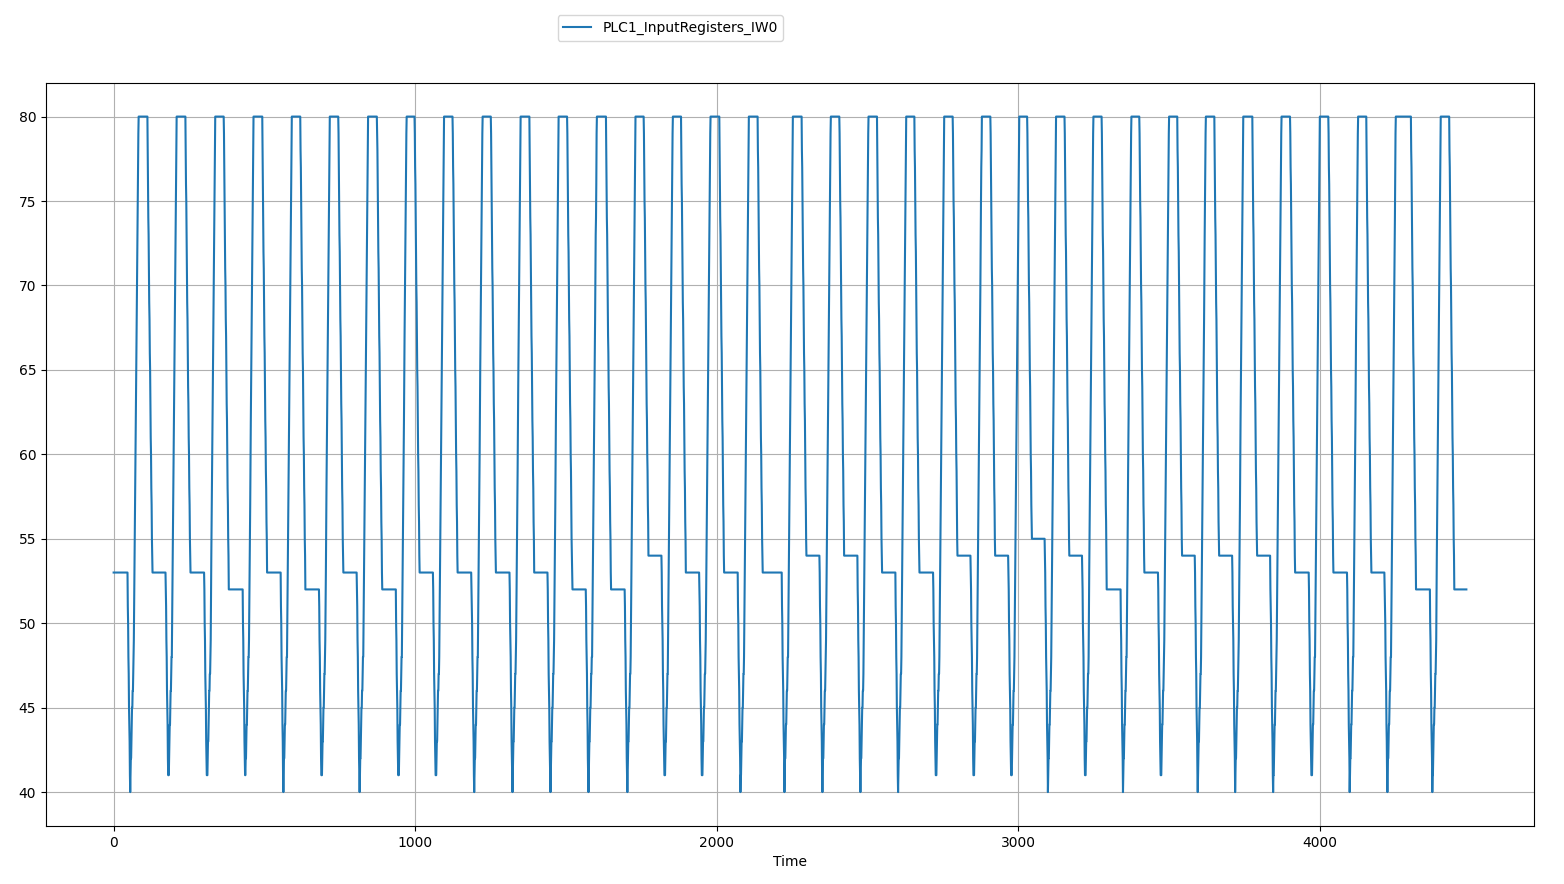
\includegraphics[width=\textwidth]{chap3/chartPlot_ceccato.png}
		\caption{Chart plot for\\ \textnormal{\texttt{PLC1\_InputRegisters\_IW01}} register}
		\label{subfig:chart_plot_ceccato}
	\end{subfigure}
	\hfill
	\begin{subfigure}{0.48\textwidth}
		\includegraphics[width=\textwidth]{chap3/histPlot_ceccato.png}
		\caption{Histogram plot for\\ \textnormal{\texttt{PLC1\_InputRegisters\_IW01}} register}
		\label{subfig:hist_plot_ceccato}
	\end{subfigure}
	\caption{Output graphs from graph analysis}
	\label{fig:ceccato_graphs}
\end{figure}

The first script plots the charts, one at the time, of certain registers entered by the user from the command line, plots in which one can see the trend of the data and get a first basic idea of what that particular register contains (a measurement, an actuation, a hardcoded setpoint, ...) and possibly the trend; the second script, instead, shows \textbf{a histogram and statistical informations} about the register entered as command-line input. These informations include:

\begin{itemize}
	\item the mean, median, standard deviation, maximum value and minimum value
	
	\item two tests for the statistical distribution: \textit{Chi-squared} test for uniformity and \textit{Shapiro-Wilk} test for normality, as shown in Listing \ref{lst:stats_anal}:

\end{itemize}

\begin{lstlisting}[language=Python,numbers=none,caption={Statistical data for \textnormal{\texttt{PLC1\_InputRegisters\_IW0}} register},label=lst:stats_anal]
	Chi-squared test for uniformity
	Distance      pvalue    Uniform?
	12488.340   0.00000000    NO    
	
	Shapiro-Wilk test for normality
	Test statistic    pvalue    Normal? 
	0.844   0.00000000    NO    
	
	Stats of PLC1_InputRegisters_IW0
	Sample mean = 60.8881; Stddev = 13.0164; max = 80; min = 40 for 4488 values
\end{lstlisting}

\subsection{Invariant Inference and Analysis}
\label{subsec:3_ceccato_invariants}
For invariant analysis Ceccato et al. rely on \textbf{Daikon} \cite{daikon_site}, a framework to \textbf{dynamically detect likely invariants} within a program. An \textit{invariant} is a property that holds at one or more points in a program, properties that are not normally made explicit in the code, but within assert statements, documentation and formal specifications: invariants are useful in understanding the behavior of a program (in our case, of the cyber physical system).

Daikon uses \textit{machine learning} techniques applied to arbitrary data with the possibility of setting custom conditions for analysis by using a specific file \cite{daikon_spinfo} with a \textit{.spinfo} extension (see Listing \ref{lst:spinfo}). The framework is designed to find the invariants of a program, with various supported programming languages, starting from the direct execution of the program itself or passing as input the execution run (typically a file in CSV format): the authors of the paper tried to apply it by analogy also to the execution runs of a cyber physical system, to extract the invariants of this system.

\begin{lstlisting}[language=Python,numbers=none,caption={Generic example of a .spinfo file for customizing rules in Daikon},label=lst:spinfo]
	PPT_NAME aprogram.point:::POINT
	VAR1 > VAR2
	VAR1 == VAR3 && VAR1 != VAR4
\end{lstlisting}

Therefore, Daikon is fed with the enriched dataset obtained in the pre-processing phase\footnote{In the paper, timestamped dataset is explicitly mentioned as input: from the tests performed, Daikon seems to ignore timestamps, hence it is indifferent whether the dataset is timestamped or not}: a simple bash script launches Daikon (optionally specifying the desired condition for analysis in the \textit{.spinfo} file), which output is simply redirected to a text file containing the general invariants of the system (i.e., valid regardless of any custom condition specified), those generated based on the custom condition in the \textit{.spinfo} file, and those generated based on the negation of the condition (see Listing \ref{lst:3_daikon_sections} below).

\begin{lstlisting}[language=Python,numbers=none,caption={The three sections of Daikon analysis outcomes},label=lst:3_daikon_sections]
	=====================================================
	aprogram.point:::POINT
	PLC2_MemoryRegisters_MW1 == PLC3_MemoryRegisters_MW1
	PLC1_MemoryRegisters_MW0 == 40.0
	PLC1_MemoryRegisters_MW1 == 80.0
	PLC1_Coils_QX00 one of { 0.0, 1.0 }
	[...]
	=====================================================
	aprogram.point:::POINT;condition="PLC1_InputRegisters_IW0 > 60"
	PLC1_InputRegisters_IW0 > PLC1_MemoryRegisters_MW0
	PLC1_InputRegisters_IW0 > PLC1_Min_safety
	PLC1_MemoryRegisters_MW0 < prev_PLC1_InputRegisters_IW0
	[...]
	=====================================================
	aprogram.point:::POINT;condition="not(PLC1_InputRegisters_IW0 > 60)"
	PLC1_InputRegisters_IW0 < PLC1_MemoryRegisters_MW1
	PLC1_InputRegisters_IW0 < PLC1_Max_safety
	PLC1_MemoryRegisters_MW1 > prev_PLC1_InputRegisters_IW0
	[...]
\end{lstlisting}
When the analysis is finished, the user is asked to enter the name of a registry to view its related invariants.\newline \newline
Some examples of invariants derived from the enriched dataset may be:

\begin{itemize}
	\item measurements bounded by some setpoint;
	
	\item actuators state changes occourred in the proximity of setpoints or, vice versa, proximity of setpoints upon the occurrence of an actuator state change;
	
	\item state invariants of some actuators correspond to a specific trend in the evolution of the measurements (ascending, descending, or stable) or, vice versa, the measurements trend corresponds to a specific state invariant of some actuators.
\end{itemize}

\subsection{Businness Process Mining and Analysis}
\label{subsec:ceccato_businessprocess}
\textit{Process mining} is the analysis of operational processes based on the event log \cite{process_mining_def}: the aim of this analysis is to \textbf{extract useful informations} from the event data to \textbf{reconstruct and understand the behavior} of the business process and how it was actually performed.\newline\newline
In the considered system, process mining begins by analyzing the event logs derived from scanning the memory registers of the PLCs and monitoring the network communications associated with the Modbus protocol, as detailed in Subsection \ref{subsec:3_scan_preproc}. These event logs serve as the \textit{execution trace} of the system. A Java program is utilized to extract and consolidate information from these event logs, resulting in a CSV format file that captures the relevant data.\newline
This file is fed to \textbf{Disco} \cite{disco}, a commercial process mining tool, which generates an \textit{activity diagram} similar to UML Activity Diagram and whose nodes represent the activities while the edges represent the relations between these activities. In Figure \ref{fig:disco_example} we can see an example of this diagram referred to PLC2 of the testbed: nodes represent the trend of register associated with measurement, actuator state changes, and communications between PLCs involving these state changes, while edges represent transitions with their associated time duration and frequency.

\begin{figure}[ht]
	\centering
	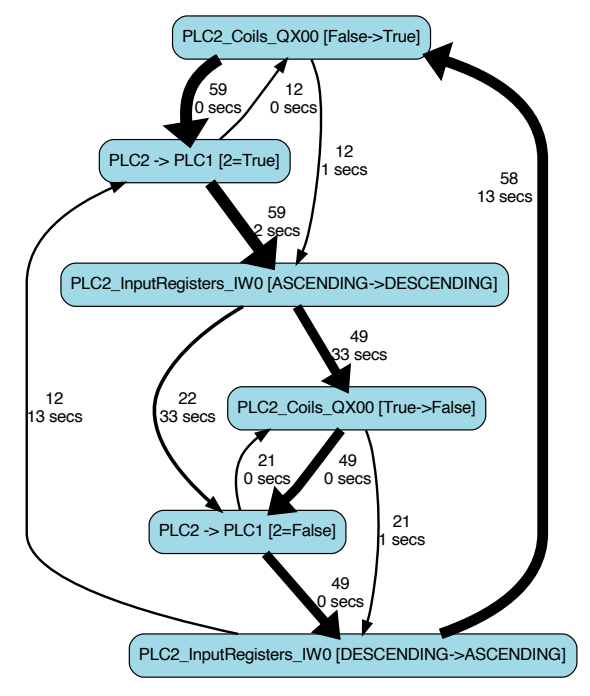
\includegraphics[scale=0.40]{chap3/disco_example.png}
	\caption{An example of Disco generated activity diagram for PLC2}
	\label{fig:disco_example}
\end{figure}

The \textit{business process} obtained in this way provides an \textbf{overview of the system} and makes it possible to \textbf{make conjectures} about its behavior, particularly between changes in actuator state and measurement trends (i.e., a given change in state of some actuators corresponds to a specific measurement trend and vice versa), and with the possibility of \textbf{establishing causality} between Modbus communications and state changes within the physical system.

\subsection{Application}
\label{subsec:ceccato_application}
In this section we will see how the black box analysis presented above in its various phases is applied in practice, using the testbed described in Subsection \ref{subsec:3_testbed}.
The methodology supports a \textbf{\textit{top-down} approach}: that is, we start with an overview of the industrial process and then gradually refine our understanding of the process by descending to a higher and higher level of detail based on the results of the previous analyses and focusing on the most interesting parts of the system for further in-depth analysis.

\paragraph{Data Collection and Pre-processing}
\label{par:3_preproc_appl} 
According to what is described in the paper, the data gathering process lasted six hours, with a granularity of one data point per second (a full system cycle takes approximately 30 minutes). Each datapoint consists of 168 attributes (55 registers plus a special register concerning the tank slope of each PLC) after the enrichment. In addition, IP addresses are automatically replaced by an abstract name identified by the prefix PLC followed by a progressive integer (PLC1, PLC2, PLC3), in order to make reading easier.

\paragraph{Graphs and Statistical Analysis}
\label{par:3_graphs_appl}
Graphs and Statistical Analysis revealed three properties regarding the contents of the registers: 

\begin{description}
	\item[\colorbox{backcolourtext}{\textnormal{\textit{Property 1:}}}] \texttt{PLC1\_MemoryRegisters\_MW0},  \texttt{PLC1\_MemoryRegisters\_MW1}, \\ \texttt{PLC2\_MemoryRegisters\_MW0},  \texttt{PLC2\_MemoryRegisters\_MW1}, \\ 
	\texttt{PLC3\_MemoryRegisters\_MW0} and 
	\texttt{PLC3\_MemoryRegisters\_MW1}
 
	registers contain constant integer values (40, 80, 10, 20, 0, 10 respectively)\footnote{From my tests on the original tool and dataset, the \texttt{PLC3\_MemoryRegisters\_MW0} register is deleted during the \textit{pre-processing} phase, as it is recognized as an unused register because of the constant value "0" it takes on. This leads me to assume that the properties are derived from a human read of the dataset prior to the \textit{pre-processing} phase.}. The authors speculate that they may be (relative) hardcoded \textbf{setpoints}.
	
	\item[\colorbox{backcolourtext}{\textnormal{\textit{Property 2:}}}] \texttt{PLC1\_Coils\_QX01}, \texttt{PLC1\_Coils\_QX02}, \texttt{PLC2\_Coils\_QX01}, \\ \texttt{PLC2\_Coils\_QX02}, \texttt{PLC3\_Coils\_QX01} and \texttt{PLC3\_Coils\_QX03} contain mutable binary (Boolean) values.
	The authors speculate that these registers can be associated with the \textbf{actuators} of the system.
	
	\item[\colorbox{backcolourtext}{\textnormal{\textit{Property 3:}}}] \texttt{PLC1\_InputRegisters\_IW0},
	\texttt{PLC2\_InputRegisters\_IW0} and \\ \texttt{PLC3\_InputRegisters\_IW0} registers contain mutable values.
\end{description}

\textit{Property 3} suggests that those registers might contain \textbf{values related to measurements}: it is therefore necessary to investigate further to see if the conjecture (referred to as \textit{Conjecture 1} in the paper) is correct.

\begin{figure}[ht]
	\centering
	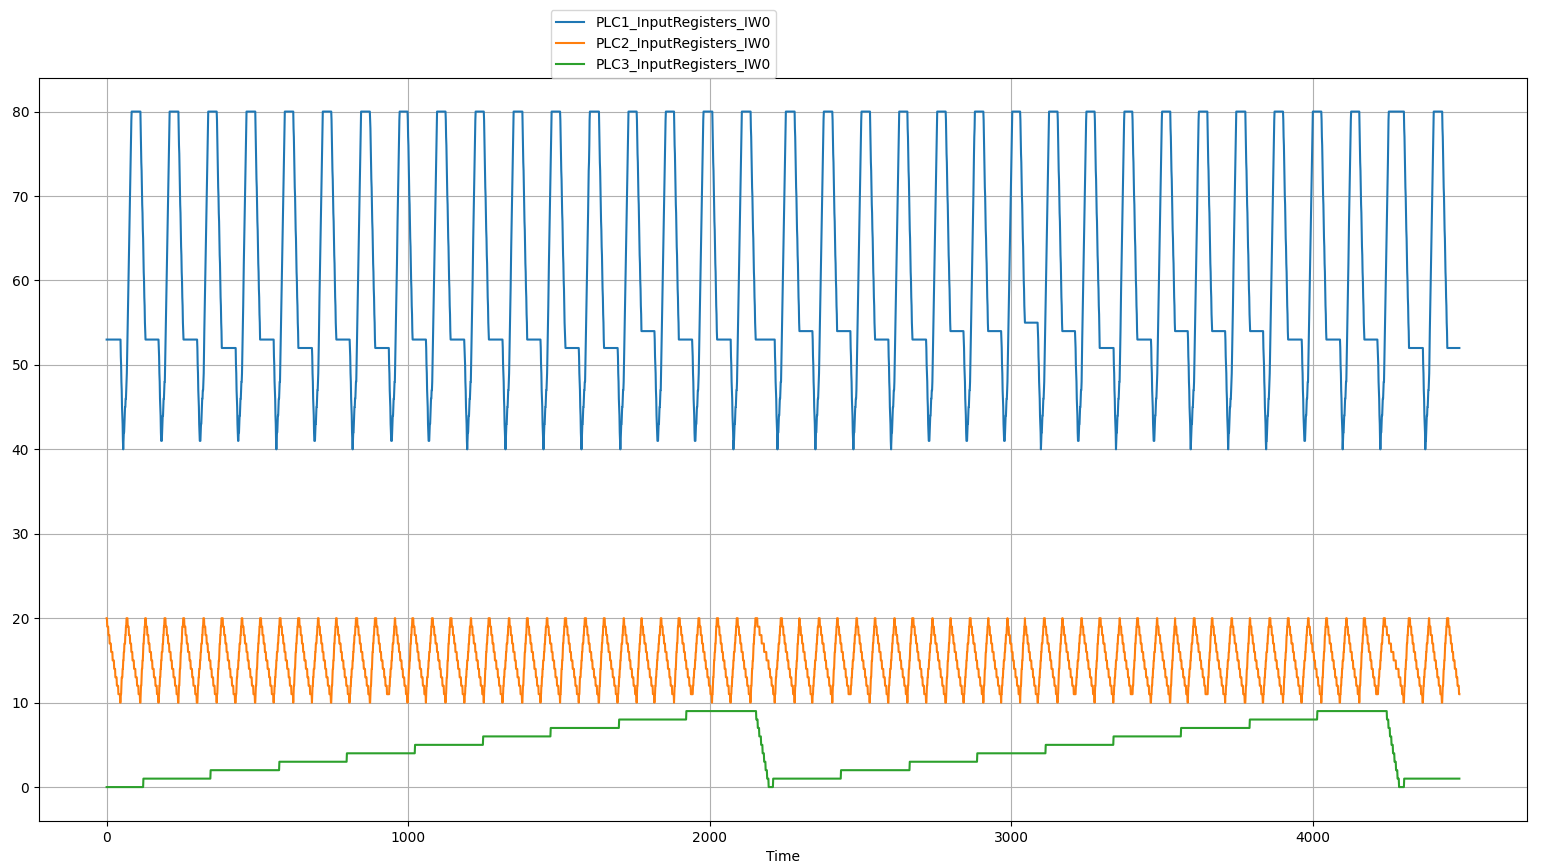
\includegraphics[scale=0.30]{chap3/graph_analysis_prop3_ceccato.png}
	\caption{Execution traces of InputRegisters\_IW0 on the three PLCs}
	\label{fig:graph_analysis_prop3}
\end{figure}

The graph analysis of the \texttt{InputRegisters\_IW0} registers of the three PLCs (summarized in Figure \ref{fig:graph_analysis_prop3} with a single plot) not only seems to confirm the conjecture, but also allows the measurements to be correlated with the contents of the \texttt{MemoryRegisters\_MW0} and \texttt{MemoryRegisters\_MW1} registers to the measurements, which may well represent the \textbf{relative setpoints of the measurements}. Hence, we have \textit{Conjecture 2} described in the paper referring to the relative setpoints:\newline\newline
\colorbox{backcolourtext}{\emph{Conjecture 2:}} 

	- the relative setpoints for \texttt{PLC1\_InputRegisters\_IW0} are 40 and 80;
	
	- the relative setpoints for \texttt{PLC2\_InputRegisters\_IW0} are 10 and 20;
	
	- the relative setpoints for \texttt{PLC3\_InputRegisters\_IW0} 0 and 9. 

\bigskip
Further confirmation of this conjecture may come from statistical analysis. Indeed, in the example in Listing 3.1, some statistical data are given for the register \texttt{PLC1\_InputRegisters\_IW0}, including the maximum value and the minimum value: these values are, in fact, 80 and 40 respectively.

\paragraph{Business Process Mining and Analysis}
\label{par:3_process_mining_appl}
With Business Process Mining, the authors aim to \textbf{visualize and highlight relevant system behaviors} by relating PLC states and Modbus commands.

\bigskip
Through analysis of the activity diagrams shown in Figure \ref{fig:business_process_cecccato}, drawn through Disco, they derive the following properties and conjectures:

\begin{description}
	\item[\colorbox{backcolourtext}{\textnormal{\textit{Property 4:}}}] PLC2 sends messages to PLC1 (see Figure \ref{subfig:pm_plc2}) which are recorded to \texttt{PLC1\_Coils\_QX02}.
	
	\item[\colorbox{backcolourtext}{\textnormal{\textit{Conjecture 3:}}}] \texttt{PLC2\_Coils\_QX00} determines the trend in tank T-202 (Figure \ref{subfig:pm_plc2}). \newline
	When this register is set to \textit{True}, the input register \texttt{PLC2\_InputRegisters\_IW0} related to the tank controlled by PLC2 starts an \textbf{ascending trend}; vice versa, when the coil register is set to \textit{False}, the input register starts a \textbf{descending trend}.
	
	\item[\colorbox{backcolourtext}{\textnormal{\textit{Conjecture 4:}}}] If \texttt{PLC1\_Coils\_QX00} change his value to True, trend in tank T-201, related to \texttt{PLC1\_InputRegisters\_IW0} and controlled by PLC1, become \textbf{ascending} (see Figure \ref{subfig:pm_plc1})

	\item[\colorbox{backcolourtext}{\textnormal{\textit{Conjecture 5:}}}] \texttt{PLC3\_Coils\_QX00} starts a \textbf{decreasing trend} in tank T-203, related to \texttt{PLC3\_InputRegisters\_IW0} and controlled by PLC3, whereas \texttt{PLC3\_Coils\_QX02} starts an \textbf{increasing trend} on the tank (see Figure \ref{subfig:pm_plc3})
\end{description}
\vfill
\pagebreak

\begin{figure}[H]
	\centering
	\begin{subfigure}{0.7\textwidth}
		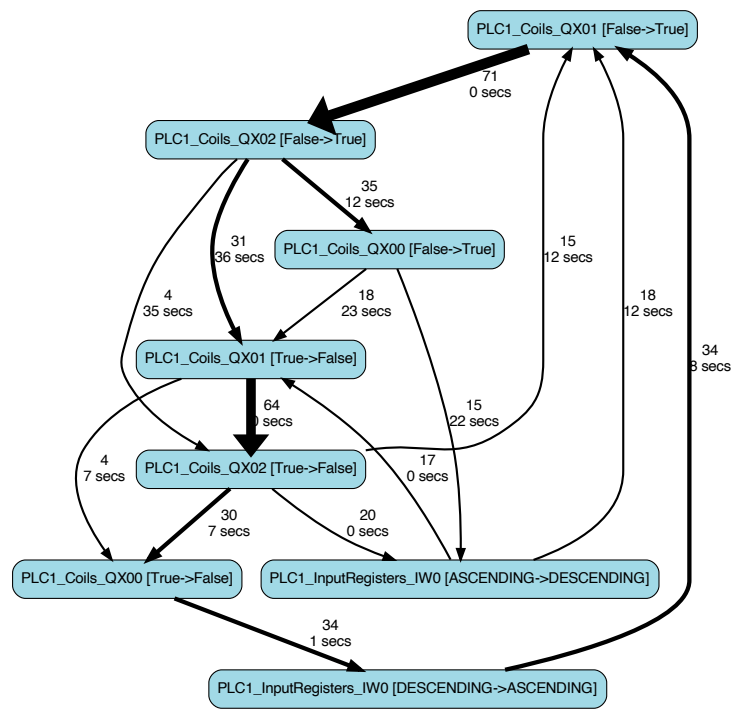
\includegraphics[width=\textwidth]{chap3/disco_plc1.png}
		\caption{States in PLC1}
		\label{subfig:pm_plc1}
	\end{subfigure}
	\hfill
	\begin{subfigure}{0.48\textwidth}
		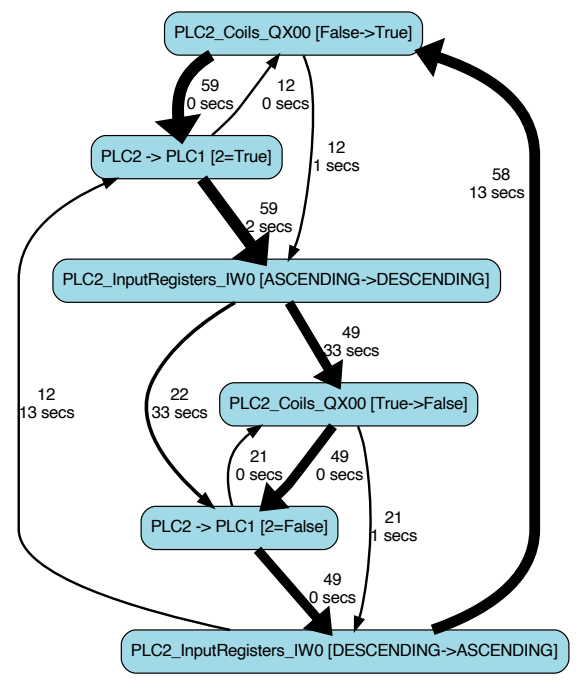
\includegraphics[width=\textwidth]{chap3/disco_plc2.png}
		\caption{States and Modbus command in PLC2}
		\label{subfig:pm_plc2}
	\end{subfigure}
	\hfill
	\begin{subfigure}{0.48\textwidth}
		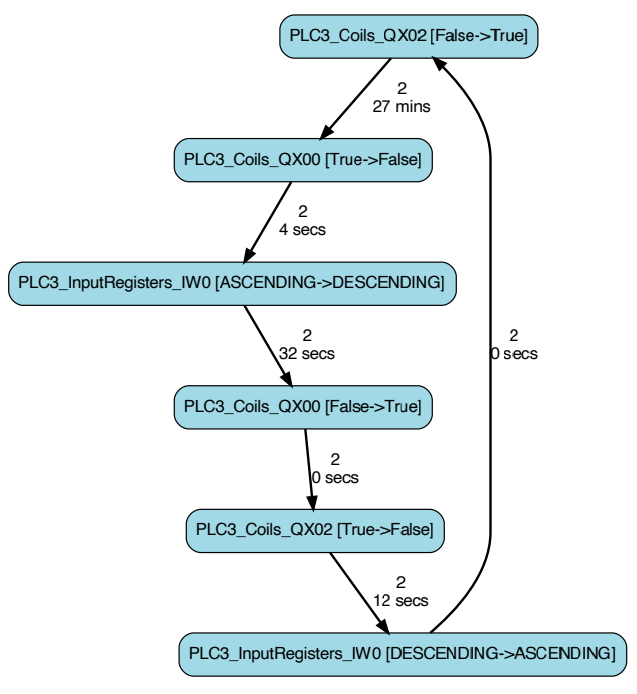
\includegraphics[width=\textwidth]{chap3/disco_plc3.png}
		\caption{States in PLC3}
		\label{subfig:pm_plc3}
	\end{subfigure}
	\caption{Business process with states and Modbus commands for the three PLCs}
	\label{fig:business_process_cecccato}
\end{figure}
\pagebreak

\paragraph{Invariant Inference and Analysis}
\label{par:3_invariant_appl}
The last phase of the analysis of the example industrial system is invariant analysis, performed through Daikon framework. At this stage, an attempt will be made to confirm what has been seen previously and to derive new properties of the system based on the results of the Daikon analysis.

\bigskip
To get gradually more and more accurate results, the authors presumably performed more than one analysis with Daikon, including certain rules within the \textit{splitter information file} (see Section \ref{subsec:3_ceccato_invariants} and Listing \ref{lst:spinfo}) based on specific conditions placed on the measurements, for example, the level of water contained in a tank. Given moreover the massive amount of invariants generated by Daikon's output, it is not easy to identify and correlate those that are actually useful for analysis: this must be done manually.

\bigskip
However, it was possible to have confirmation of the conjectures made in the previous stages of the analysis: starting with the setpoints, analyzing the output of the invariants returned by Daikon\footnote{The invariants shown here are a manual summary and derivation of those actually returned in output by Daikon. We will discuss this more in Section \ref{subsec:3_ceccato_limitations}} reveals that \newline \newline
\small\texttt{PLC1\_InputRegisters\_IW0 >= PLC1\_MemoryRegisters\_MW0 == 40.0}\\
\texttt{PLC1\_InputRegisters\_IW0 <= PLC1\_MemoryRegisters\_MW1 == 80.0}\\
\texttt{PLC2\_InputRegisters\_IW0 >= PLC2\_MemoryRegisters\_MW0 == 10.0}\\
\texttt{PLC2\_InputRegisters\_IW0 <= PLC2\_MemoryRegisters\_MW1 == 20.0}\\
\texttt{PLC3\_InputRegisters\_IW0 >= PLC3\_MemoryRegisters\_MW0 == 0.0}\\
\texttt{PLC3\_InputRegisters\_IW0 <= PLC3\_MemoryRegisters\_MW1 == 9.0} \newline \newline
\normalsize i.e., that the \texttt{MemoryRegisters\_MW0} and \texttt{MemoryRegisters\_MW1} registers of each PLC contain the \textbf{absolute minimum and maximum setpoints}, respectively (\textit{Property 5}).

\bigskip
There is also a confirmation regarding \textit{Property 4}: from the computed invariants it can be seen that \newline \newline
\small\texttt{PLC1\_Coils\_QX01 == PLC1\_Coils\_QX02 == PLC2\_Coils\_QX00}\newline \newline
\normalsize and from this derive that there is a \textbf{communication channel between PLC2 and PLC1}, where the value of \texttt{PLC2\_Coils\_QX00} is copied to \texttt{PLC1\_Coils\_QX01} and \texttt{PLC1\_Coils\_QX02} (\textit{Property 6}).

\bigskip
Regarding the \textbf{relationships between actuator state changes and measurement trends}, invariant analysis yields the results summarized in the following rules:

\begin{description}
	\item[\colorbox{backcolourtext}{\normalfont\textit{Property 7:}}] Tank T-202 level \textit{increases} iff \texttt{PLC1\_Coils\_QX01 == True}. Otherwise, if \texttt{PLC1\_Coils\_QX01 == False} will be \textit{non-increasing}.
\end{description}
	This is because if the coil is \textit{True} the condition \newline \scriptsize\texttt{PLC2\_InputRegisters\_IW0 == PLC2\_MemoryRegisters\_MW0 == 20.0 \&\& PLC2\_slope > 0} \newline \normalsize is verified. 
	On the opposite hand, if the coil is \textit{False}, the condition \newline \scriptsize\texttt{PLC2\_InputRegisters\_IW0 == PLC2\_MemoryRegisters\_MW0 == 20.0 \&\& PLC2\_slope <= 0}  \normalsize is verified. The \textit{slope} is increasing if > 0, decreasing if < 0, stable otherwise.

\begin{description}
	\item[\colorbox{backcolourtext}{\normalfont\textit{Property 8:}}] Tank T-201 level \textit{increases} iff \texttt{PLC1\_Coils\_QX00 == True}. On the other hand, if \texttt{PLC1\_Coils\_QX00 == False} and if \texttt{PLC1\_Coils\_QX01 == True} the level will be \textit{non-decreasing}.
	
	\item[\colorbox{backcolourtext}{\normalfont\textit{Property 9:}}] Tank T-203 level \textit{decreases} iff \texttt{PLC3\_Coils\_QX00 == True}. It will be \textit{non-decreasing} if \texttt{PLC1\_Coils\_QX00 == False}.
\end{description}

The last two properties concern the \textbf{relationship between actuator state changes and the setpoints}: it is intended to check what happens to the actuators when the water level reaches one of these setpoints. From the analysis of the relevant invariants, the following properties are derived:

\begin{description}
	\item[\colorbox{backcolourtext}{\normalfont\textit{Property 10:}}] Tank T-201 reaches the upper absolute setpoint when\\ \texttt{PLC1\_Coils\_QX00} changes its state from \textit{True} to \textit{False}. If the coil changes from \textit{False} to \textit{True}, the tank reaches its absolute lower setpoint.
	
	\item[\colorbox{backcolourtext}{\normalfont\textit{Property 11:}}]
	Tank T-203 reaches the upper absolute setpoint when\\ \texttt{PLC3\_Coils\_QX00} changes its state from \textit{True} to \textit{False}. If the coil changes from \textit{False} to \textit{True}, the tank reaches its absolute lower setpoint.	 
\end{description}

\subsection{Limitations}
\label{subsec:3_ceccato_limitations}
The methodology proposed by Ceccato et al. is certainly valid and offers a good starting point for approaching the reverse engineering of an industrial control system from the attacker's perspective, while also providing a tool to perform this task.

\bigskip
The limitations of this approach, however, all lie in the tool mentioned above and also in the testbed described in Section \ref{subsec:3_testbed}. In this section we will explain which are the criticisms of each phase, while in Chapter 4 we will formulate proposals to improve and make this methodology more efficient.

\paragraph{General Criticism}
\label{par:3_limit_ceccato_general}
There are several critical aspects associated with the application of this approach: the primary one concerns the fact that the proposed tool seems to be built specifically for the testbed used and that it is not applicable to other contexts, even to the same type of industrial control system (water treatment systems, in this case). 

\bigskip
What severely limits the analysis performed with the tool implemented by Ceccato et al. is the use of \textit{ad hoc} solutions and \textit{a posteriori} interventions done manually on the datasets after the data gathering process: we will discuss this last aspect in more detail later.\newline
Moreover, there is the presence of many \textit{hardcoded} variables and conditions within the scripts: this makes the system unconfigurable and unable to properly perform the various stages of the analysis as errors can occur due to incorrect data and mismatches with the system under analysis.\newline
Having considered, furthermore, only the Modbus protocol for network communications between the PLCs is another major limiting factor and does not help the methodology to be adaptable to different systems communicating with different protocols (sometimes even multiple ones on the same system). 

\bigskip
Let us now look at the limitations and critical aspects of each phase.

\paragraph{Testbed}
\label{par:3_testbed_limitations}
The testbed environment used by Ceccato et. al is entirely simulated, from the physical system to the control system. The PLCs were built with \textbf{OpenPLC} \cite{openplc} in a Docker environment \cite{docker}, while the physics part was built through \textbf{Simulink} \cite{simulink}.

\bigskip
OpenPLC is an open source cross-platform software that simulates the hardware and software functionality of a physical PLC and also offers a complete editor for PLC program development with support for all standard languages: \textit{Ladder Logic} (LD), \textit{Function Block Diagram} (FBD), \textit{Instruction List} (IL), \textit{Structured Text} (ST), and \textit{Sequential Function Chart} (SFC).\newline
It is for sure an excellent choice for creating a zero-cost industrial or home automation and \textit{Internet of Things} (IoT) system that is easy to manage via a dedicated, comprehensive and functional web interface. In spite of these undoubted merits, however, there are (at the moment) \textbf{very few supported protocols}: the main one and also referred to in the official documentation is \textbf{Modbus}, while the other protocol is DNP3.

\begin{description}
	\item[\emph{\underline{First limitation}}] The biggest problem with the testbed, however, is not with the controller part, but with the \textbf{physical part}: first of all, it must be said that although this is something purely demonstrative even though it is fully functional, the implemented Simulink model is really \textbf{oversimplified} compared to the iTrust SWaT system, which itself is a scaled-down version of a real water treatment plant. In fact, in the entire system there are only three actuators, two of which are connected to the same tank and controlled by the same PLC, and sensors related only to the water level in the system's tanks: in a real system there are many more \textit{field devices}, which can monitor and control other aspects of the system beyond the mere contents of the tanks. Consider, for example, measuring and controlling the chemicals in the water, the pressure of the liquid in the filter unit, or more simply the amount of water flow at a given point or time.\newline
	All these must be considered and represent a number of additional variables that makes analysis and consequently reverse engineering of the system more difficult.
	
	\item[\emph{\underline{Second limitation}}] The second critical aspect concerns the \textbf{simulation of the physics of the liquid} inside the tanks: Simulink does not consider the fact that inside a tank that is filling (emptying) the liquid in it undergoes \textbf{fluctuations} which cause the level sensor not to see the water level constantly increasing (decreasing) or at most being stable at each point of detection. Figure \ref{fig:testbed_physics} exemplifies more clearly with an example the concept just expressed: these oscillations cause a \textbf{perturbation} in the data.\newline
	This issue leads to the difficulty, on a real physical system, of \textbf{correctly calculating the trend of a measurement} by using the slope attribute: if this was obtained with a too low granularity, the trend will be oscillating between increasing and decreasing even when in reality this would be in general increasing (decreasing) or stable; on the other hand, if the slope was obtained with a too high granularity there is a loss of information and the trend may be "flattened" with respect to reality.\newline
	In the present case, the slope in the Simulink model was calculated statically with a (very) low granularity, 5 and 6 seconds according to the Properties 7 and 9 described in the original paper: an averagely careful reader will have already guessed that this granularity is inapplicable to the real system in Figure \ref{subfig:real_physics}. As we will later see, we need to \textbf{operate on the data perturbations} to be able to obtain a suitable granularity and a correct calculation of the slope and consequently of the measurement trend.
\end{description}
\vfill

\pagebreak
\begin{figure}[ht]
	\centering
	\begin{subfigure}{0.9\textwidth}
		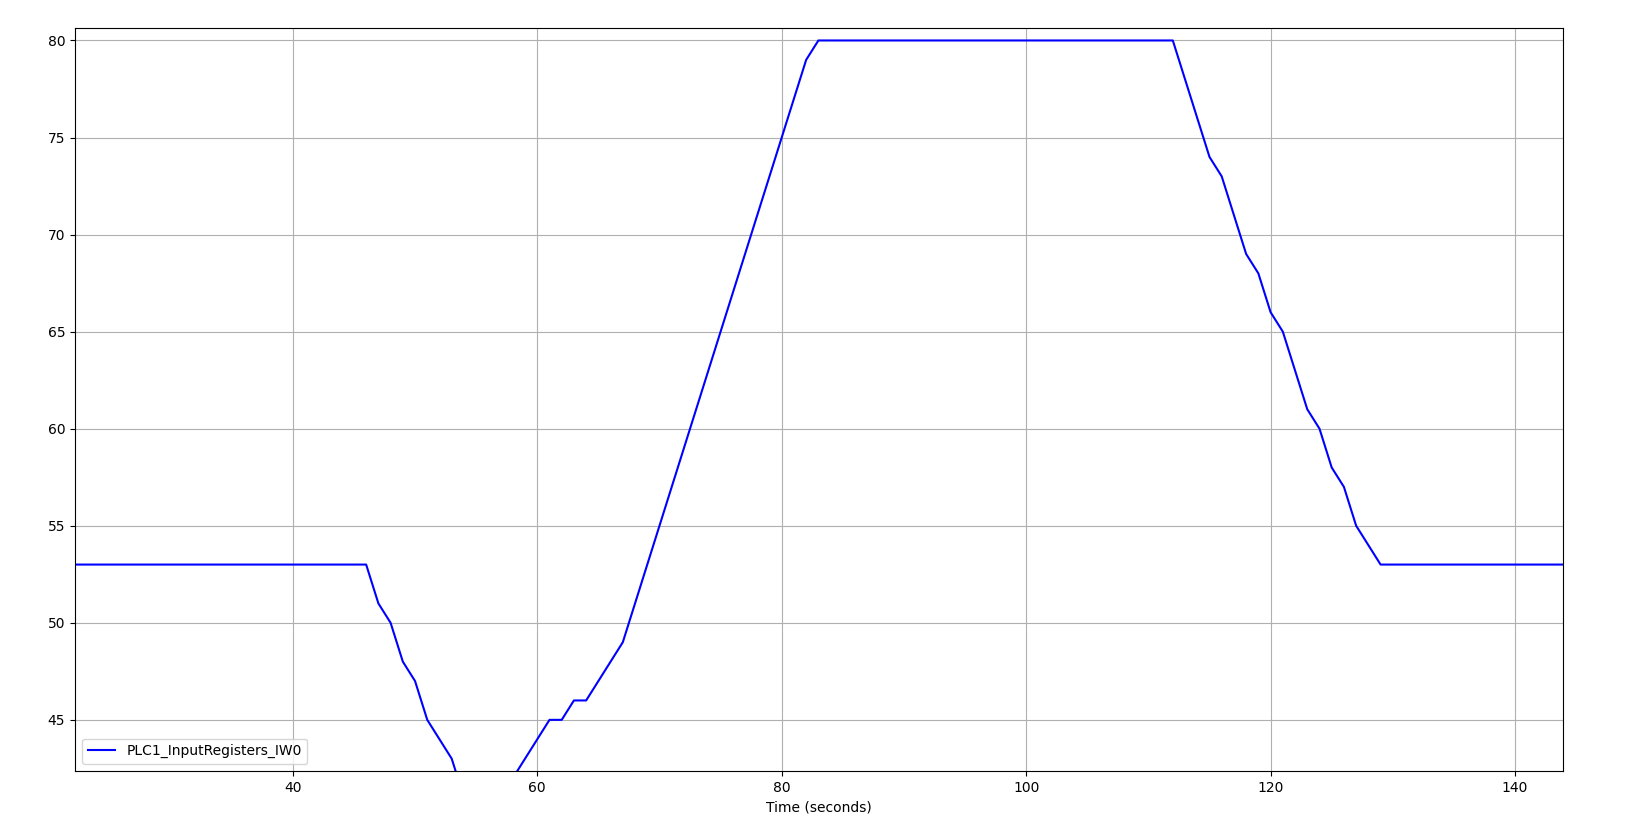
\includegraphics[width=\textwidth]{chap3/simulink_physics.png}
		\caption{}
		\label{subfig:simulink_physics}
	\end{subfigure}
	\hfill
	\begin{subfigure}{0.9\textwidth}
		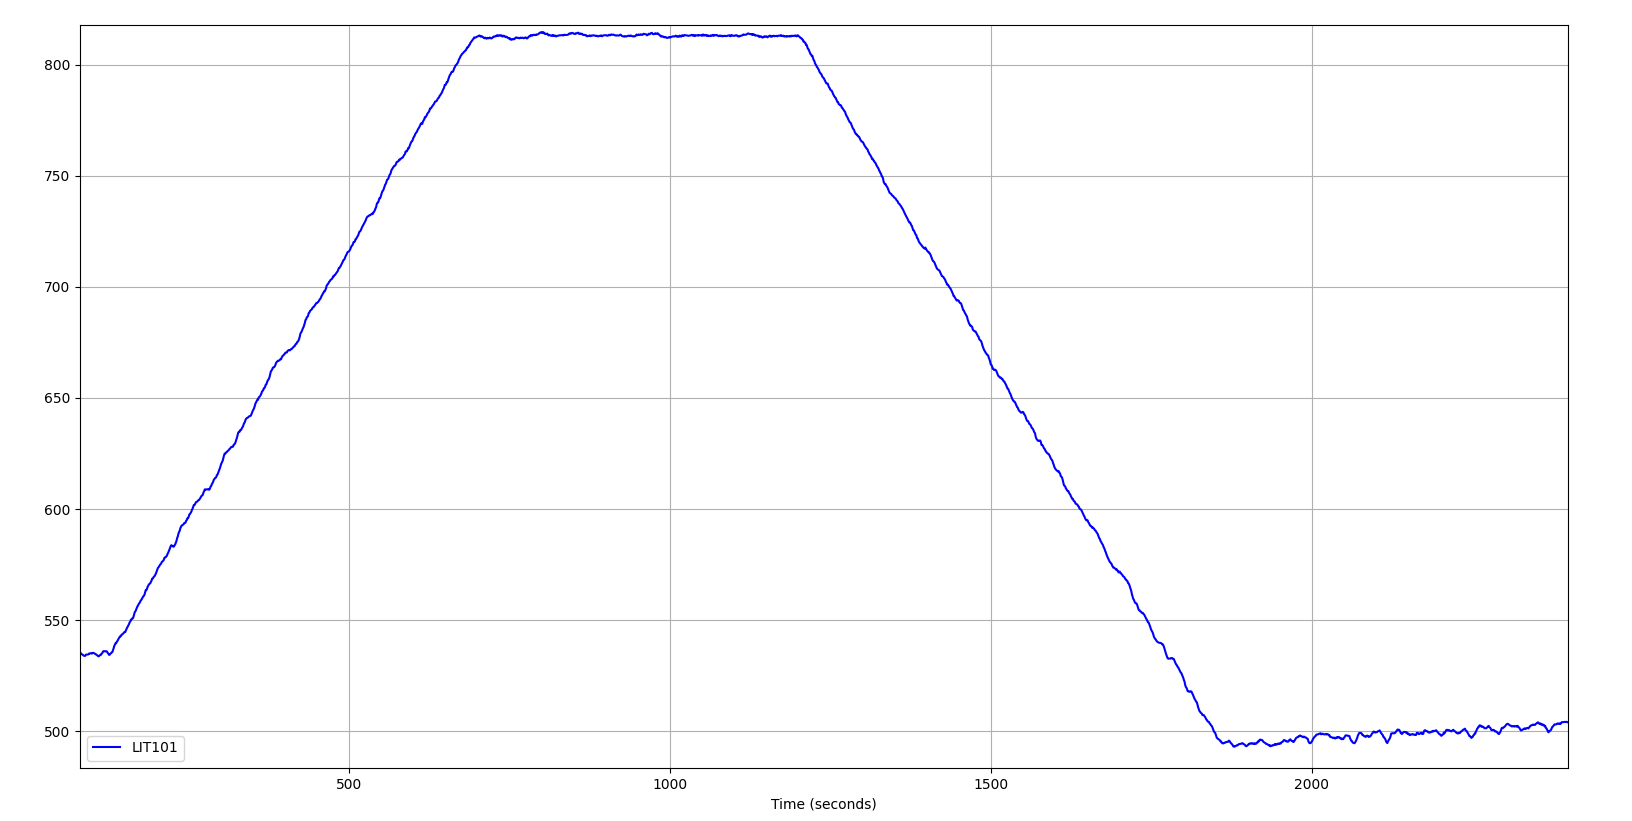
\includegraphics[width=\textwidth]{chap3/real_physics.png}
		\caption{}
		\label{subfig:real_physics}
	\end{subfigure}
	\caption{Water physics compared: simulated physics in the Simulink model (a) and physics in a real system (iTrust SWaT) (b). Fluctuations in the tank level in (b), almost completely absent in (a), can be appreciated.}
	\label{fig:testbed_physics}
\end{figure}

\paragraph{Pre-processing}
\label{par:3_preproc_limitation}
In the pre-processing phase, the authors make use of a Python script to merge all the datasets of the individual PLCs into a single dataset, remove the (supposedly) unused registers, and finally enrich the obtained dataset with additional attributes. These attributes, as seen in \ref{par:3_preproc}, are:

\begin{itemize}
	\item the \textbf{previous value} of all registers;
	
	\item some \textbf{additional relative setpoints} named \texttt{PLC\textit{x}\_Max\_safety} and\\ 
	\texttt{PLC\textit{x}\_Min\_safety} (where \textit{x} is the PLC number), which represent a kind of alert on reaching the maximum and minimum water levels of the tanks;
	
	\item the \textbf{measurement slope}.	
\end{itemize}

\begin{description}
	\item[\emph{\underline{First limitation}}] Merging the datasets of all individual PLCs into a single dataset representing the entire system can be a sound practice if the system to be anlized is (very) small as is the testbed analyzed here, consisting of a few PLCs and especially a few registers. If, however, the complexity of the system increases, this type of merging can become counterproductive and make it difficult to analyze and understand the data obtained in subsequent steps.\newline
	In short, there is no possibility to analyze only a subsystem and thus make the analysis faster and more understandable. Moreover, a data gathering can take up to days, and the analyst/attacker may need to make an analysis of the system isolating precise time ranges, ignoring everything that happens before and/or after: all of this, with the tool we have seen, cannot be done.

	\item[\emph{\underline{Second limitation}}] Regarding the additional attributes, looking at the code of the script that performs the enrichment, we observed that \textbf{some attributes were manually inserted} after the merging phase: we are referring in particular to the attributes \texttt{PLC\textit{x}\_Max\_safety} and \texttt{PLC\textit{x}\_Min\_safety}, whose references were moreover hardcoded into the script, and the \textit{slope} whose calculation method we mentioned in the previous paragraph about the testbed limitations.\newline
	In the end, only the attribute \textit{prev} related to the value at the previous point of the detection is inserted automatically for all registers, moreover without the possibility to choose whether this attribute should be extended to all registers or only to a part.
\end{description}

\paragraph{Graphs and Statistical Analysis}
\label{par:3_graphs_limitations}
Describing the behavior of graphical analysis in Section \ref{subsec:3_graph_analysis} we had already mentioned that only one register plot at a time was shown and not, for example, a single window containing the charts of all registers entered by the user as input from the command line, such as in Figure \ref{fig:graph_analysis_prop3}. Figure \ref{fig:3_ceccato_graphs_behavior} shows the actual behavior of graphical analysis: note that although we have specified four registers (highlighted in red in the figures) as command-line parameters, only one at a time is shown and it is necessary to close the current chart in order to display the next one.

\begin{figure}[ht]
	\centering
	\begin{subfigure}{0.48\textwidth}
		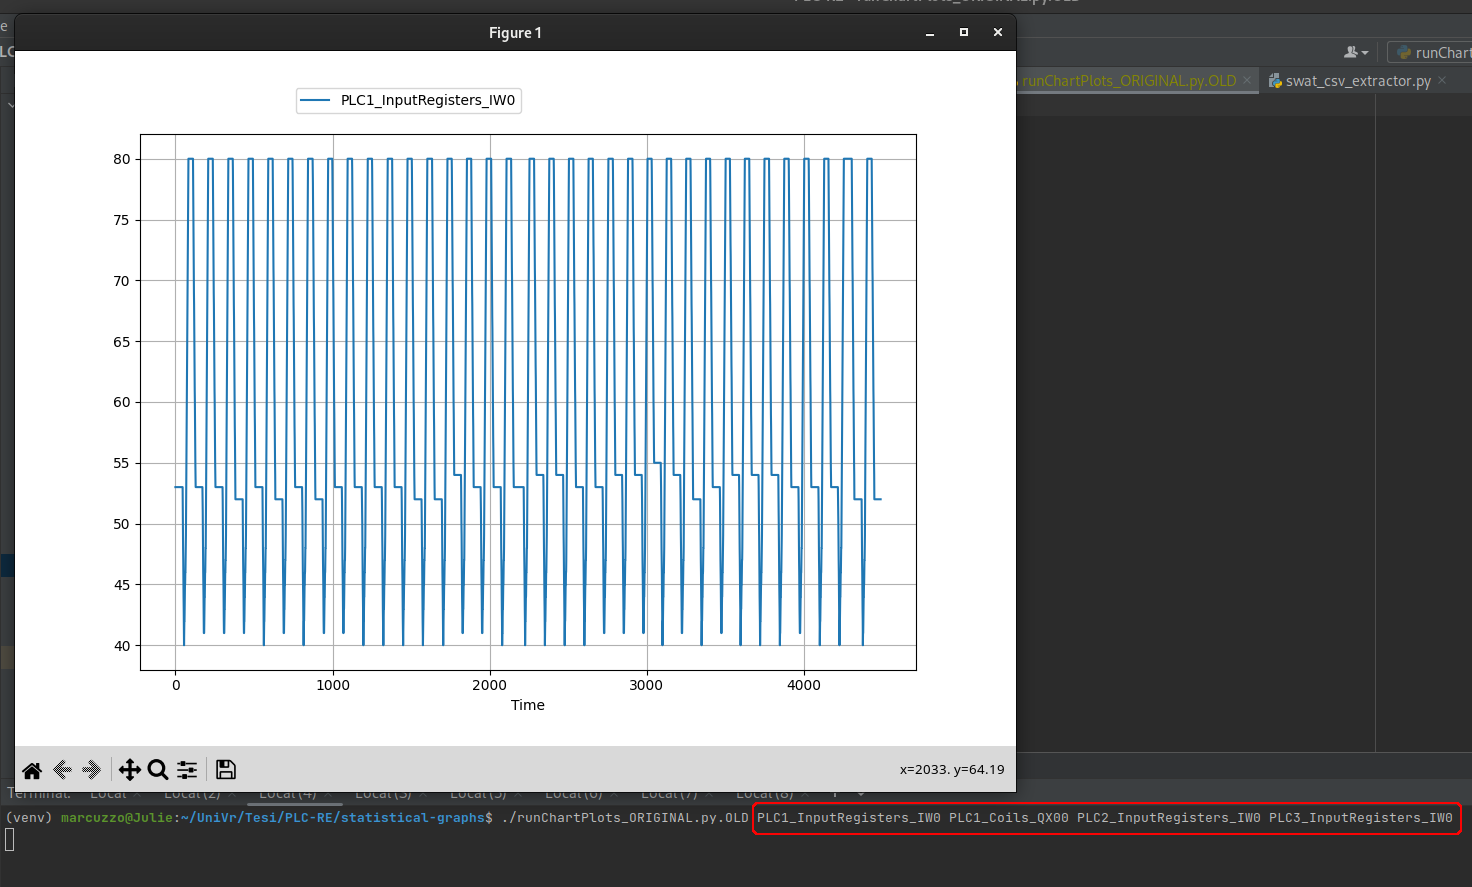
\includegraphics[width=\textwidth]{chap3/plot_ceccato1.png}
		\caption{Chart for \texttt{PLC1\_InputRegisters\_IW0}}
		\label{subfig:3_real_plot_ceccato_1}
	\end{subfigure}
	\hfill
	\begin{subfigure}{0.48\textwidth}
		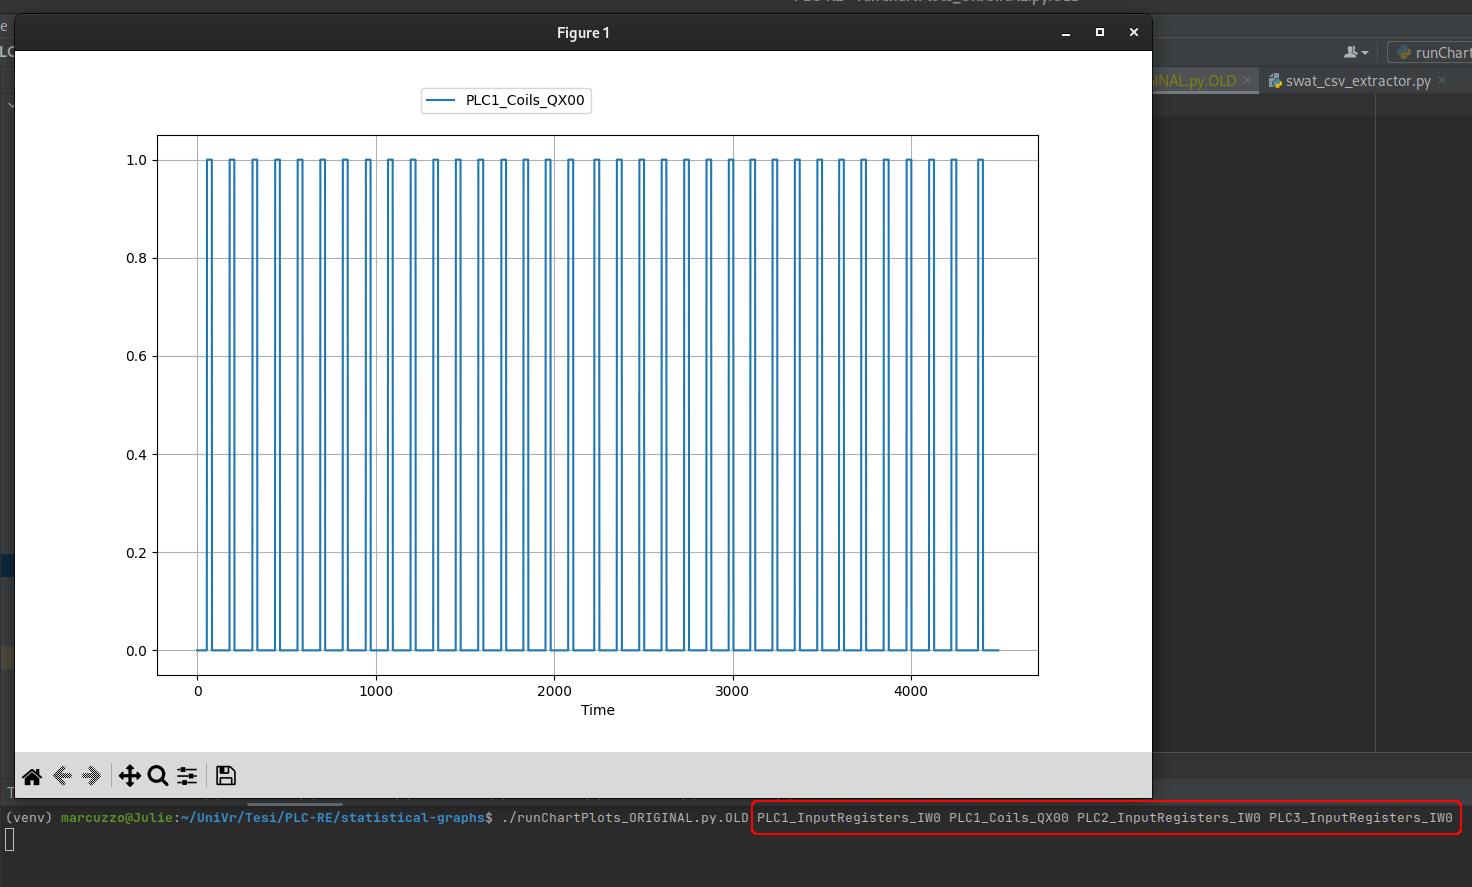
\includegraphics[width=\textwidth]{chap3/plot_ceccato2.png}
		\caption{Chart for \texttt{PLC1\_Coils\_QX00}}
		\label{subfig:3_real_plot_ceccato_2}
	\end{subfigure}
	\caption{Behavior of the Graph Analysis on the Ceccato et al.'s tool}
	\label{fig:3_ceccato_graphs_behavior}
\end{figure}

\begin{description}
	\item[\emph{\underline{First limitation}}] While displaying charts for individual registers still provides useful information about the system such as the distinction between actuators and measurements and the general trend of the latter, single display does not allow one to catch, or at least makes it difficult, the relationship that exists between actuators and measurements, where it exists, because a view of the system as a whole is missing.\newline
	In this way, the risk is to make conjectures about the behavior of the system that may prove to be at least imprecises, if not inaccurates.

	\item[\emph{\underline{Second limitation}}] On the other hand, regarding the statistical analysis, two observations need to be made: the first is that for the given system, I personally was unable to appreciate the usefulness of the generated histogram in Figure \ref{subfig:hist_plot_ceccato}, as it does not provide any particular new information that has not already been obtained from the graphical analysis (except maybe something marginal); the second observation pertains to the presentation of statistical information obtained from the histogram plot. In certain cases, the histogram plot itself can overshadow the displayed statistical information. These statistics are actually shown on the terminal from which the script is executed. However, to an inattentive or unfamiliar user, these statistics may be mistaken for debugging output or warnings, as they coincide with the display of the histogram plot window, which takes the focus (see Figure \ref{fig:3_hist_plot_fail}).\newline

	\begin{figure}[ht]
		\centering
		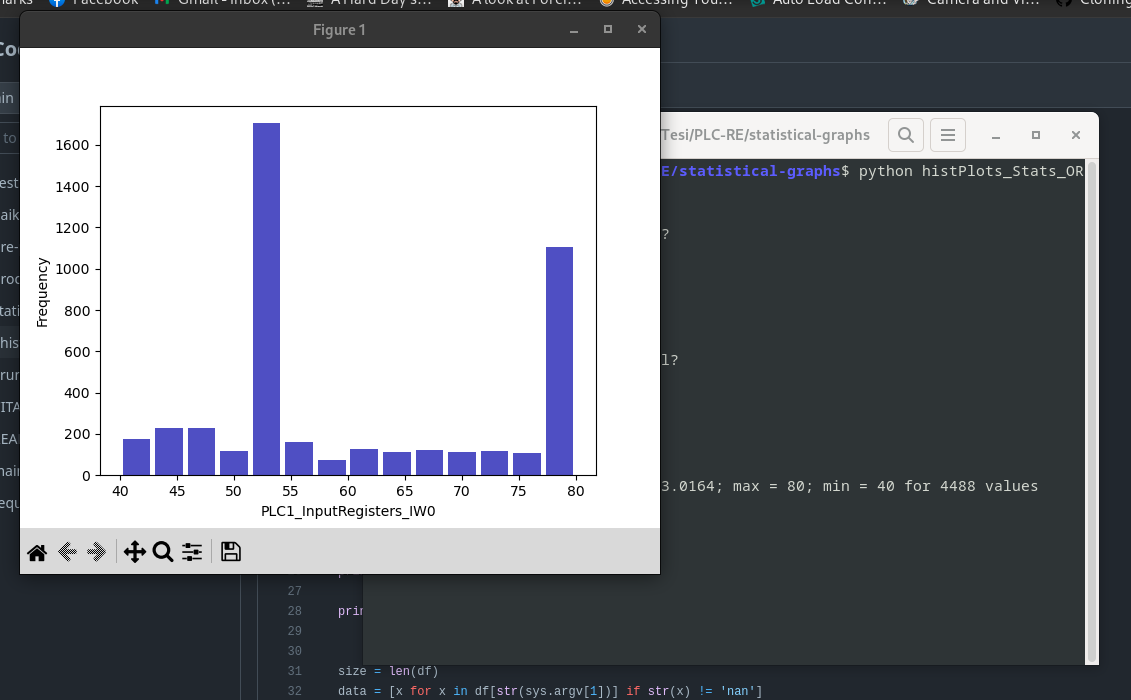
\includegraphics[scale=0.30]{chap3/hist_plot_fail.png}
		\caption{Histogram plot overshadowing statistical information shown on the terminal window in the background}
		\label{fig:3_hist_plot_fail}
	\end{figure}

	\noindent In general, however, little statistical information is provided.
\end{description}

\paragraph{Business Process Mining and Analysis}
\label{par:3_processmining_limitations}
Concerning the data mining, this is a purely ad \textit{hoc solution}, designed to work under special conditions: first, the timestamped dataset of the physical process and the one obtained after the packet sniffing operation of Modbus traffic on the network need to be synchronized and have the same granularity, in this case one event per second.\newline
It is relatively easy, therefore, to find correspondences between Modbus commands sent over the network and events occurring on the physical system, such as state changes in actuations, due in part to the fact that the number of communications over the network is really small (see Section \ref{subsec:3_testbed}).

\begin{description}
	\item[\emph{\underline{First limitation}}] In a real system, network communications are much more numerous and involve many more devices even in the same second: finding the exact correspondence with what is happening in the cyber physical system becomes much more difficult.\newline
	Since this is, as mentioned, an \textit{ad hoc} solution, only the Modbus protocol is being considered: as widely used as this industrial protocol is, other protocols that are widely used \cite{protocols_market_shares} such as EtherNet/IP (see Section \ref{subsubsec:enip}) or Profinet should be considered in order to extend the analysis to other industrial systems that use a different communication network.
	
	\item[\emph{\underline{Second limitation}}] The other limiting aspect of the business process mining phase is the \textbf{process mining software} used to generate the activity diagram. As mentioned in Section \ref{subsec:ceccato_businessprocess}, the process mining software used by Ceccato et al. is \textbf{Disco}: this is commercial software, with an academic license lasting only 30 days (although free of charge), released for Windows and MacOS operating systems only, which makes its use under Linux systems impossible except by using emulation environments such as Wine.\newline
	For what is my personal vision and training as a computer scientist, it would have been preferable to use a \textit{cross-platform}, \textit{freely licensed open source} software alternative to Disco: one such software could have been \textbf{ProM Tools} \cite{prom_tools}, a framework for process mining very similar to Disco in functionality, but fitting the criteria just described, or use Python libraries such as \textbf{PM4PY} \cite{pm4py}, which offer ready-to-use algorithms suitable for various process mining needs.
\end{description}
\vfill

\paragraph{Invariants Inference and Analysis}
\label{par:3_invariant_limitations}
The limitation in this case is principally Daikon: this software is designed to compute the invariants of a software from its live execution or from a file containing its execution flow, not to find the invariants of a cyber physical system. Since there are currently no better consolidated alternatives for inferring invariants, however, an attempt was still made to use Daikon as best as possible.

\begin{figure}[ht]
	\centering
	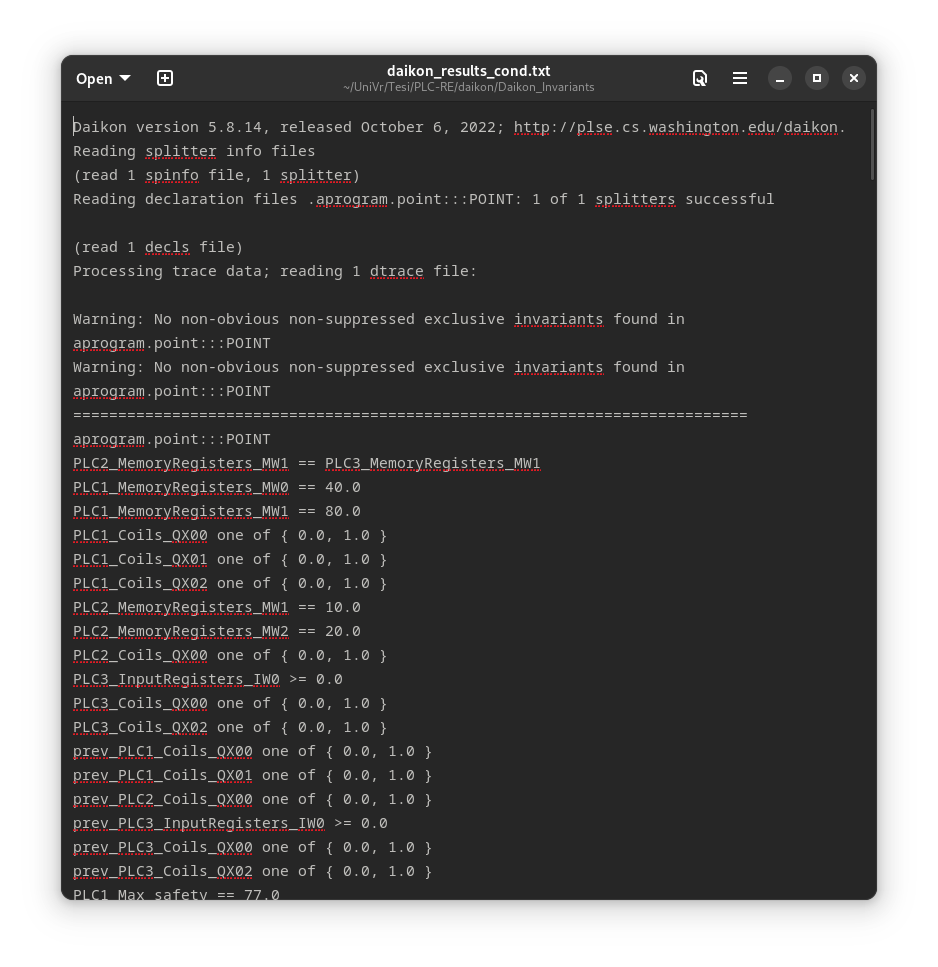
\includegraphics[scale=0.35]{chap3/daikon_output_ceccato.png}
	\caption{Example of Daikon's output}
	\label{fig:daikon_output_ceccato}
\end{figure}

\begin{description}
	\item[\emph{\underline{First limitation}}] The biggest problem with Daikon applied to the computation of invariants of an industrial system is the difficult reading of the resulting output: the software in fact returns a very long list of invariants, one invariant per line, many of no use and without correlating invariants that may have common features or deriving additional information from them. The process of screening and recognizing the significant invariants, as well as the correlation between them, must be done by a human: certainly not an easy task given the volume of invariants one could theoretically be faced with (hundreds and hundreds of invariants). An example of Daikon's output can be seen in Figure \ref{fig:daikon_output_ceccato}.

	\item[\emph{\underline{Second limitation}}] The bash script used in this phase of the analysis does not help at all in deriving significant invariants more easily: it merely launches Daikon and saves its output to a text file by simply redirecting the stdout to file. No data reprocessing is done during this step. In addition, if a condition is to be specified to Daikon before performing the analysis, it is necessary each time to edit the .spinfo file by manually entering the desired rule, an inconvenient operation when multiple analyses are to be performed with different conditions each time. 
\end{description}
Table \ref{table:3_ceccato_limitations_table} provides a summary of the limitations discussed regarding the Ceccato et al. framework.

{\small
\begin{longtable}[c]{| l | l |}
	\hline
	\textbf{Phase} & \textbf{Limitations} \\ [0.5ex] 
	\hline
	\multirow{4}{12em}{Testbed} & - Oversimplified model compared to \\
	& iTrust SWaT system \\
	& - Physics of the liquid not considered: this \\ 
	& causes data perturbation \\
	\hline
	\multirow{5}{12em}{Pre-processing} & - It is not possible to select \\
	& a subsystem by (groups of) PLCs or by \\
	& time range \\
	& - Some additional attributes are manually \\
	& inserted in the dataset \\
	\hline 
	\multirow{6}{12em}{Graphical/Statistical Analysis} & - Only one chart at the time \\
	& is displayed: difficulty in capturing  the \\ 
	& relationship between actuators and \\
	& sensors \\
	& - Statistical Analysis provides little \\ 
	& information \\
	\hline
	\multirow{4}{12em}{Business Process Analysis} & - Ad hoc solution designed to \\
	& work under special conditions \\
	& - Use of commercial software for process \\
	& mining \\
	\hline
	\multirow{3}{12em}{Invariant Analysis} & - Reading output is challenging  \\
	& - Script for analysis merely launches \\
	& Daikon without reprocessing outcomes \\
	\hline
	%\multirow{3}{4em}{\textbf{Priority}} & Confidentiality  \\
	%& Integrity  \\
	%& Availability  \\
	%\hline
	
	\caption{Summary table of Ceccato et al. framework limitations}
	\label{table:3_ceccato_limitations_table}
\end{longtable}
}
\vfill
\nolinenumbers
